%======================================================================
\chapter{Proces Twórczy}
%======================================================================

Niniejszy rozdział opisuje proces twórczy stojący za projektem \textit{Echoes of Vanitas} – od koncepcji fabularnej i projektu świata, przez decyzje artystyczne, aż po wstępne szkice postaci. Podejście twórcze zakłada pełną autorskość wszystkich elementów – fabuły, grafiki oraz projektu rozgrywki.

\section{Zarys Fabuły}
%----------------------------------------------------------------------

Akcja gry toczy się w alternatywnym, średniowiecznym świecie zamieszkałym wyłącznie przez inteligentne zwierzęta. Świat ten – mimo braku technologicznego odpowiednika naszego – posiada własną historię, kultury i hierarchie społeczne. Ludzkie cywilizacje dawno wymarły, a ich pamięć stała się tabu lub legendą.

Głównym bohaterem jest \textbf{Nietoperz Złodziej} – samotnik mieszkający na skraju lasu, który utrzymuje się z drobnych kradzieży i prowadzi baczną obserwację świata z ukrycia. Pewnego dnia, nieopodal swojej chatki, natrafia na starą, zakurzoną księgę zapisaną w nieznanym języku. Zaintrygowany tajemnicą postanawia odkryć jej pochodzenie i treść.

W miarę tłumaczenia i badania księgi Nietoperz stopniowo odkrywa, że język należał do dawno wymarłej rasy – ludzi. W świecie gry nikt nie pamięta już o ich istnieniu; sama idea człowieka jest mitem lub zakazaną legendą. Bohater wplątuje się w serię wydarzeń prowadzących go przez zapomnianych ruiny, pałace zwierzęcych monarchów oraz ukryte miejsca dawnej ludzkiej cywilizacji.

Fabuła zakłada liczne zwroty akcji, tajemnice i moralne wybory, które zmieniają sposób postrzegania przeszłości przez bohatera. Gracz staje się świadkiem odradzającej się pamięci o ludzkości i odkrywa, dlaczego dominująca niegdyś rasa zniknęła. Wiedza zawarta w księdze niesie zarówno potencjał, jak i zagrożenie – a każda decyzja gracza kształtuje kierunek historii.

Narracja prowadzona jest w sposób nieliniowy – gracz decyduje, które wątki eksploruje w pierwszej kolejności. System questów zapewnia strukturę narracyjną, dzieląc fabułę na główne zadania (questów głównych) i poboczne wątki (questów pobocznych), które wzbogacają wiedzę o świecie i postaciach.

\section{Projekt Świata Gry}
%----------------------------------------------------------------------

Świat \textit{Echoes of Vanitas} podzielony jest na kilka typów regionów, odzwierciedlających różnorodność ekosystemów i kultur zamieszkałych przez zwierzęta:

\begin{itemize}
    \item \textbf{Skraj lasu} – punkt startowy, dom bohatera. Środowisko bujnej, nieco tajemniczej roślinności, w którym toczy się wczesna część gry.
    \item \textbf{Miasto zwierząt} – centrum handlowe i społeczne regionu, zamieszkałe przez różnorodne gatunki. Tu gracz może przyjmować zadania od NPC, handlować i rozwijać fabułę.
    \item \textbf{Ruiny ludzkiej cywilizacji} – niebezpieczne, zapomniane miejsca pełne pułapek i wrogich stworzeń. Kluczowe dla głównego wątku fabularnego.
    \item \textbf{Pałace monarchów} – rozbudowane, strzeżone siedziby władców. Wymagają od gracza dyplomacji lub skradania się.
\end{itemize}

Środowisko gry zaprojektowane jest w stylu 2.5D – plansze tworzone są z elementów trójwymiarowych (modele Blender), lecz rozgrywka odbywa się na płaszczyźnie dwuwymiarowej. Taki zabieg pozwala na bogate, przestrzenne tło przy zachowaniu klasycznej mechaniki platformówki RPG.

\section{Koncepcje Postaci}
%----------------------------------------------------------------------

\subsection{Główny Bohater – Nietoperz Złodziej}

Projekt wizualny głównego bohatera łączy cechy charakterystyczne dla nietoperza (skrzydła używane jako płaszcz, duże uszy, nocny tryb życia) z estetyką złodzieja-awanturnika ze świata fantasy. Postać przeszła kilka iteracji szkicowych, zanim osiągnęła finalny wygląd.

\begin{figure}[h]
    \centering
    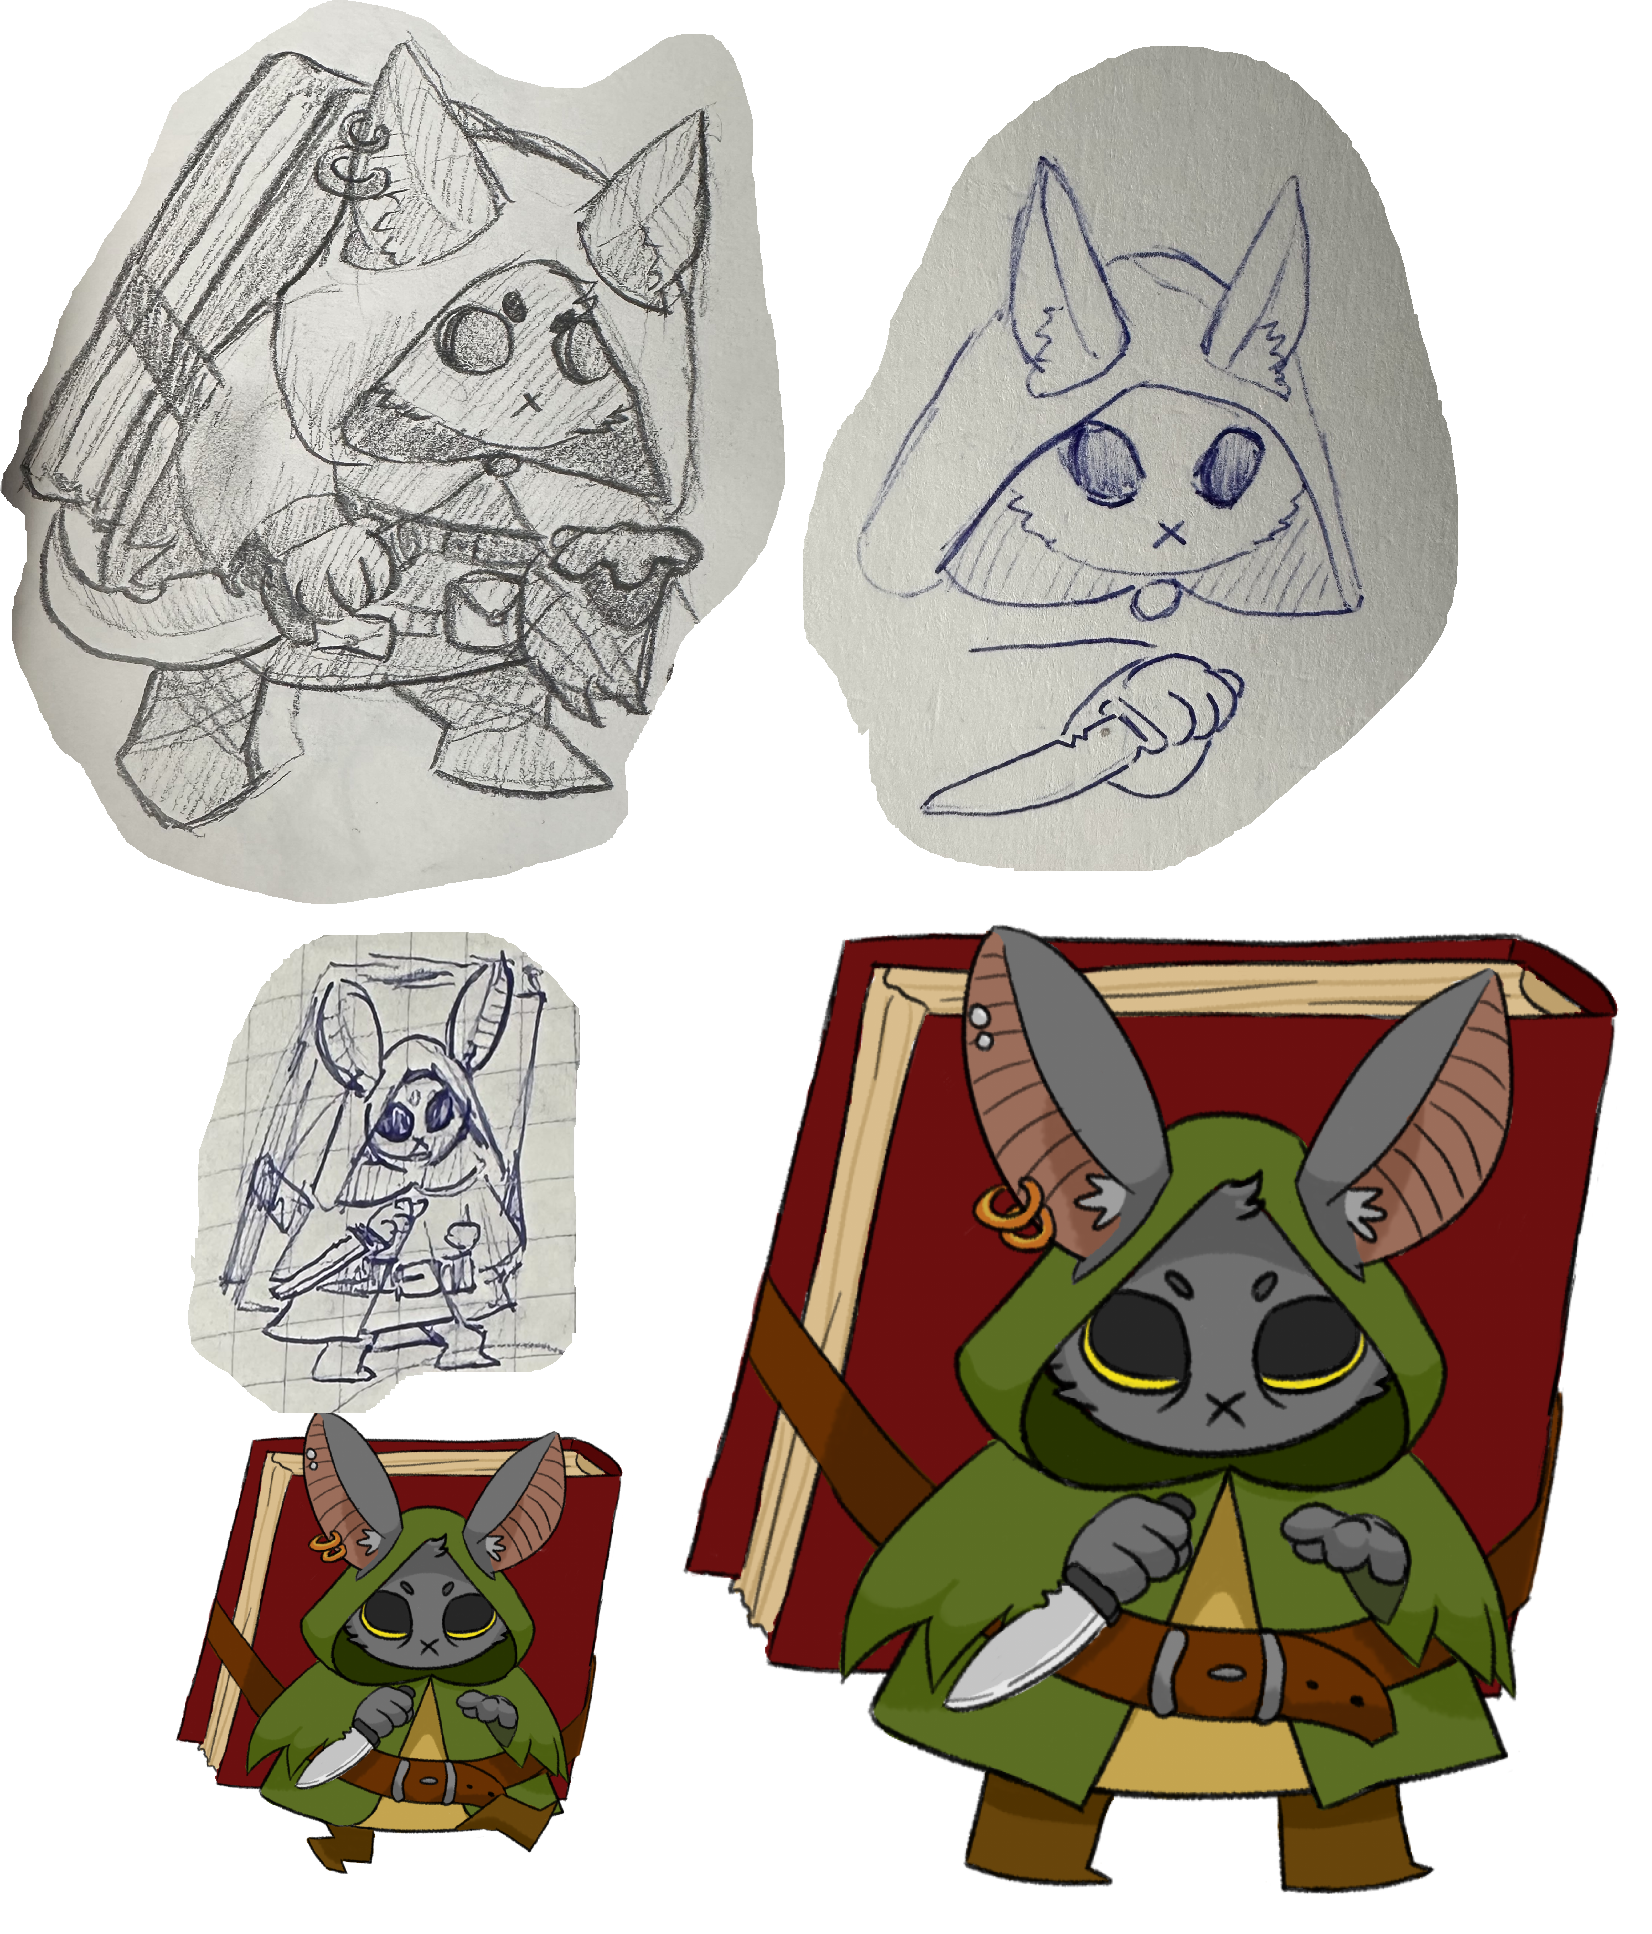
\includegraphics[width=0.75\textwidth]{images/bat-design.png}
    \caption{Źródło własne: Wczesne szkice koncepcyjne postaci Nietoperza Złodzieja oraz postać końcowa. Wykonane w Clip Studio Paint.}
    \label{fig:bat-design}
\end{figure}

Pod względem mechanicznym, Nietoperz Złodziej posiada następujące atrybuty:
\begin{itemize}
    \item \textbf{Zdrowie (Health)} – punkty życia postaci,
    \item \textbf{Siła (Strength)} – wpływa na obrażenia zadawane podczas ataku,
    \item \textbf{Złoto (Gold)} – waluta używana do handlu i ulepszania ekwipunku,
    \item \textbf{Doświadczenie (Experience)} – zdobywane za pokonanie wrogów i ukończenie questów.
\end{itemize}

Postać może być wyposażona w przedmioty z pięciu slotów: hełm, naszyjnik, sztylet, buty i strona (magiczny zwój).

\subsection{NPC – Labrador Rycerz}

Jednym z pierwszych projektów NPC jest postać strażnika przy bramie miasta – Labrador Rycerz. Łączy on wierność i niezłomność rasy Labrador Retriever z estetyką rycerza w zbroi gotycko-fantasy.

\begin{figure}[h]
    \centering
    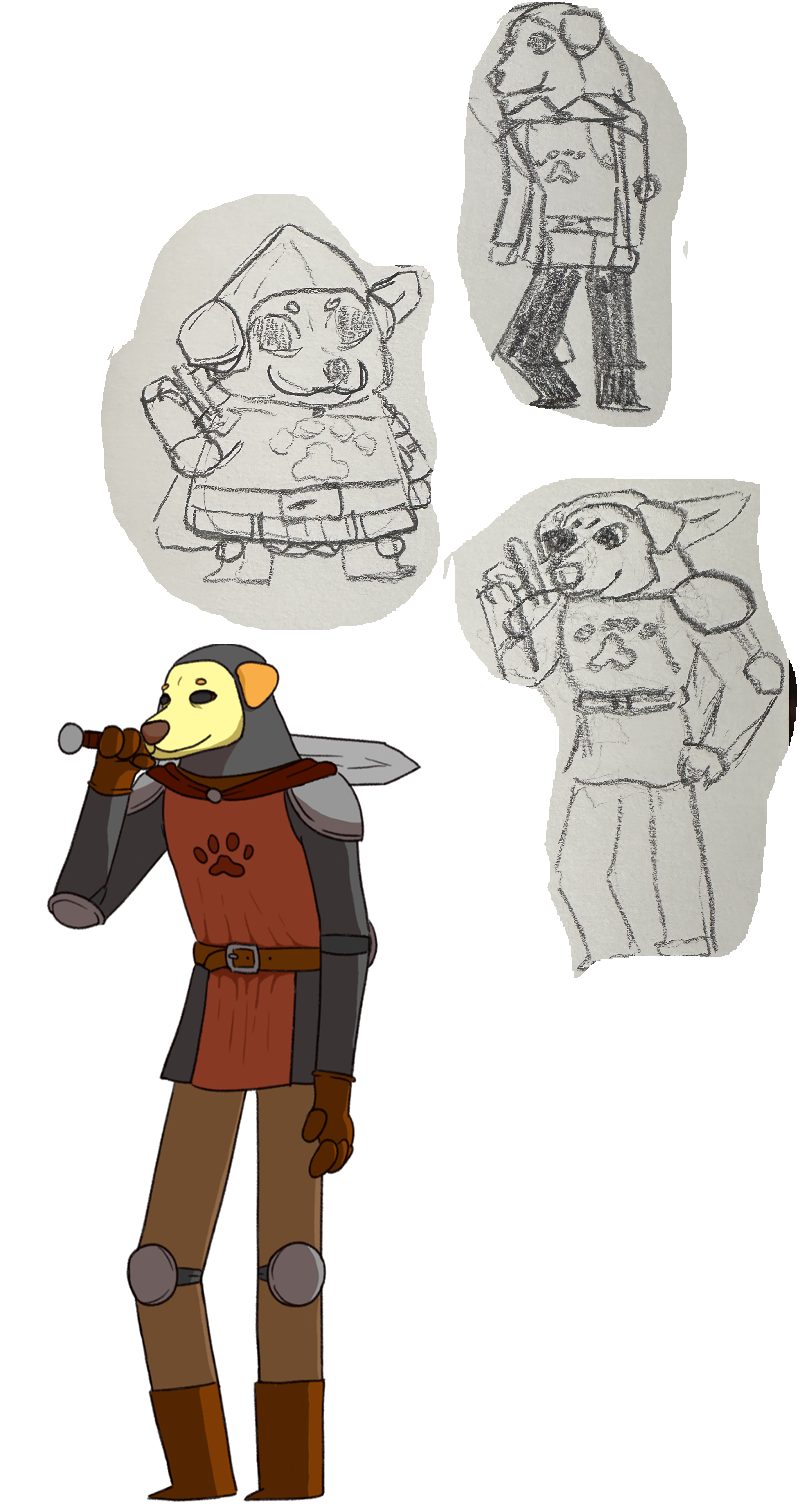
\includegraphics[width=0.75\textwidth]{images/labra_knight.png}
    \caption{Źródło własne: Wczesne szkice koncepcyjne postaci NPC strażnika (Labrador Rycerz) oraz końcowy design. Wykonane w Clip Studio Paint.}
    \label{fig:labra-knight}
\end{figure}

\subsection{Wstępny Zarys Stylu Postaci}

Poniższy rysunek przedstawia wstępny zarys koncepcji postaci niegrywalnych w odniesieniu do lokacji, w których się pojawiają. Każda lokacja ma własną paletę kolorów i styl ubioru postaci, co pozwala na szybkie orientowanie się w świecie.

\begin{figure}[h]
    \centering
    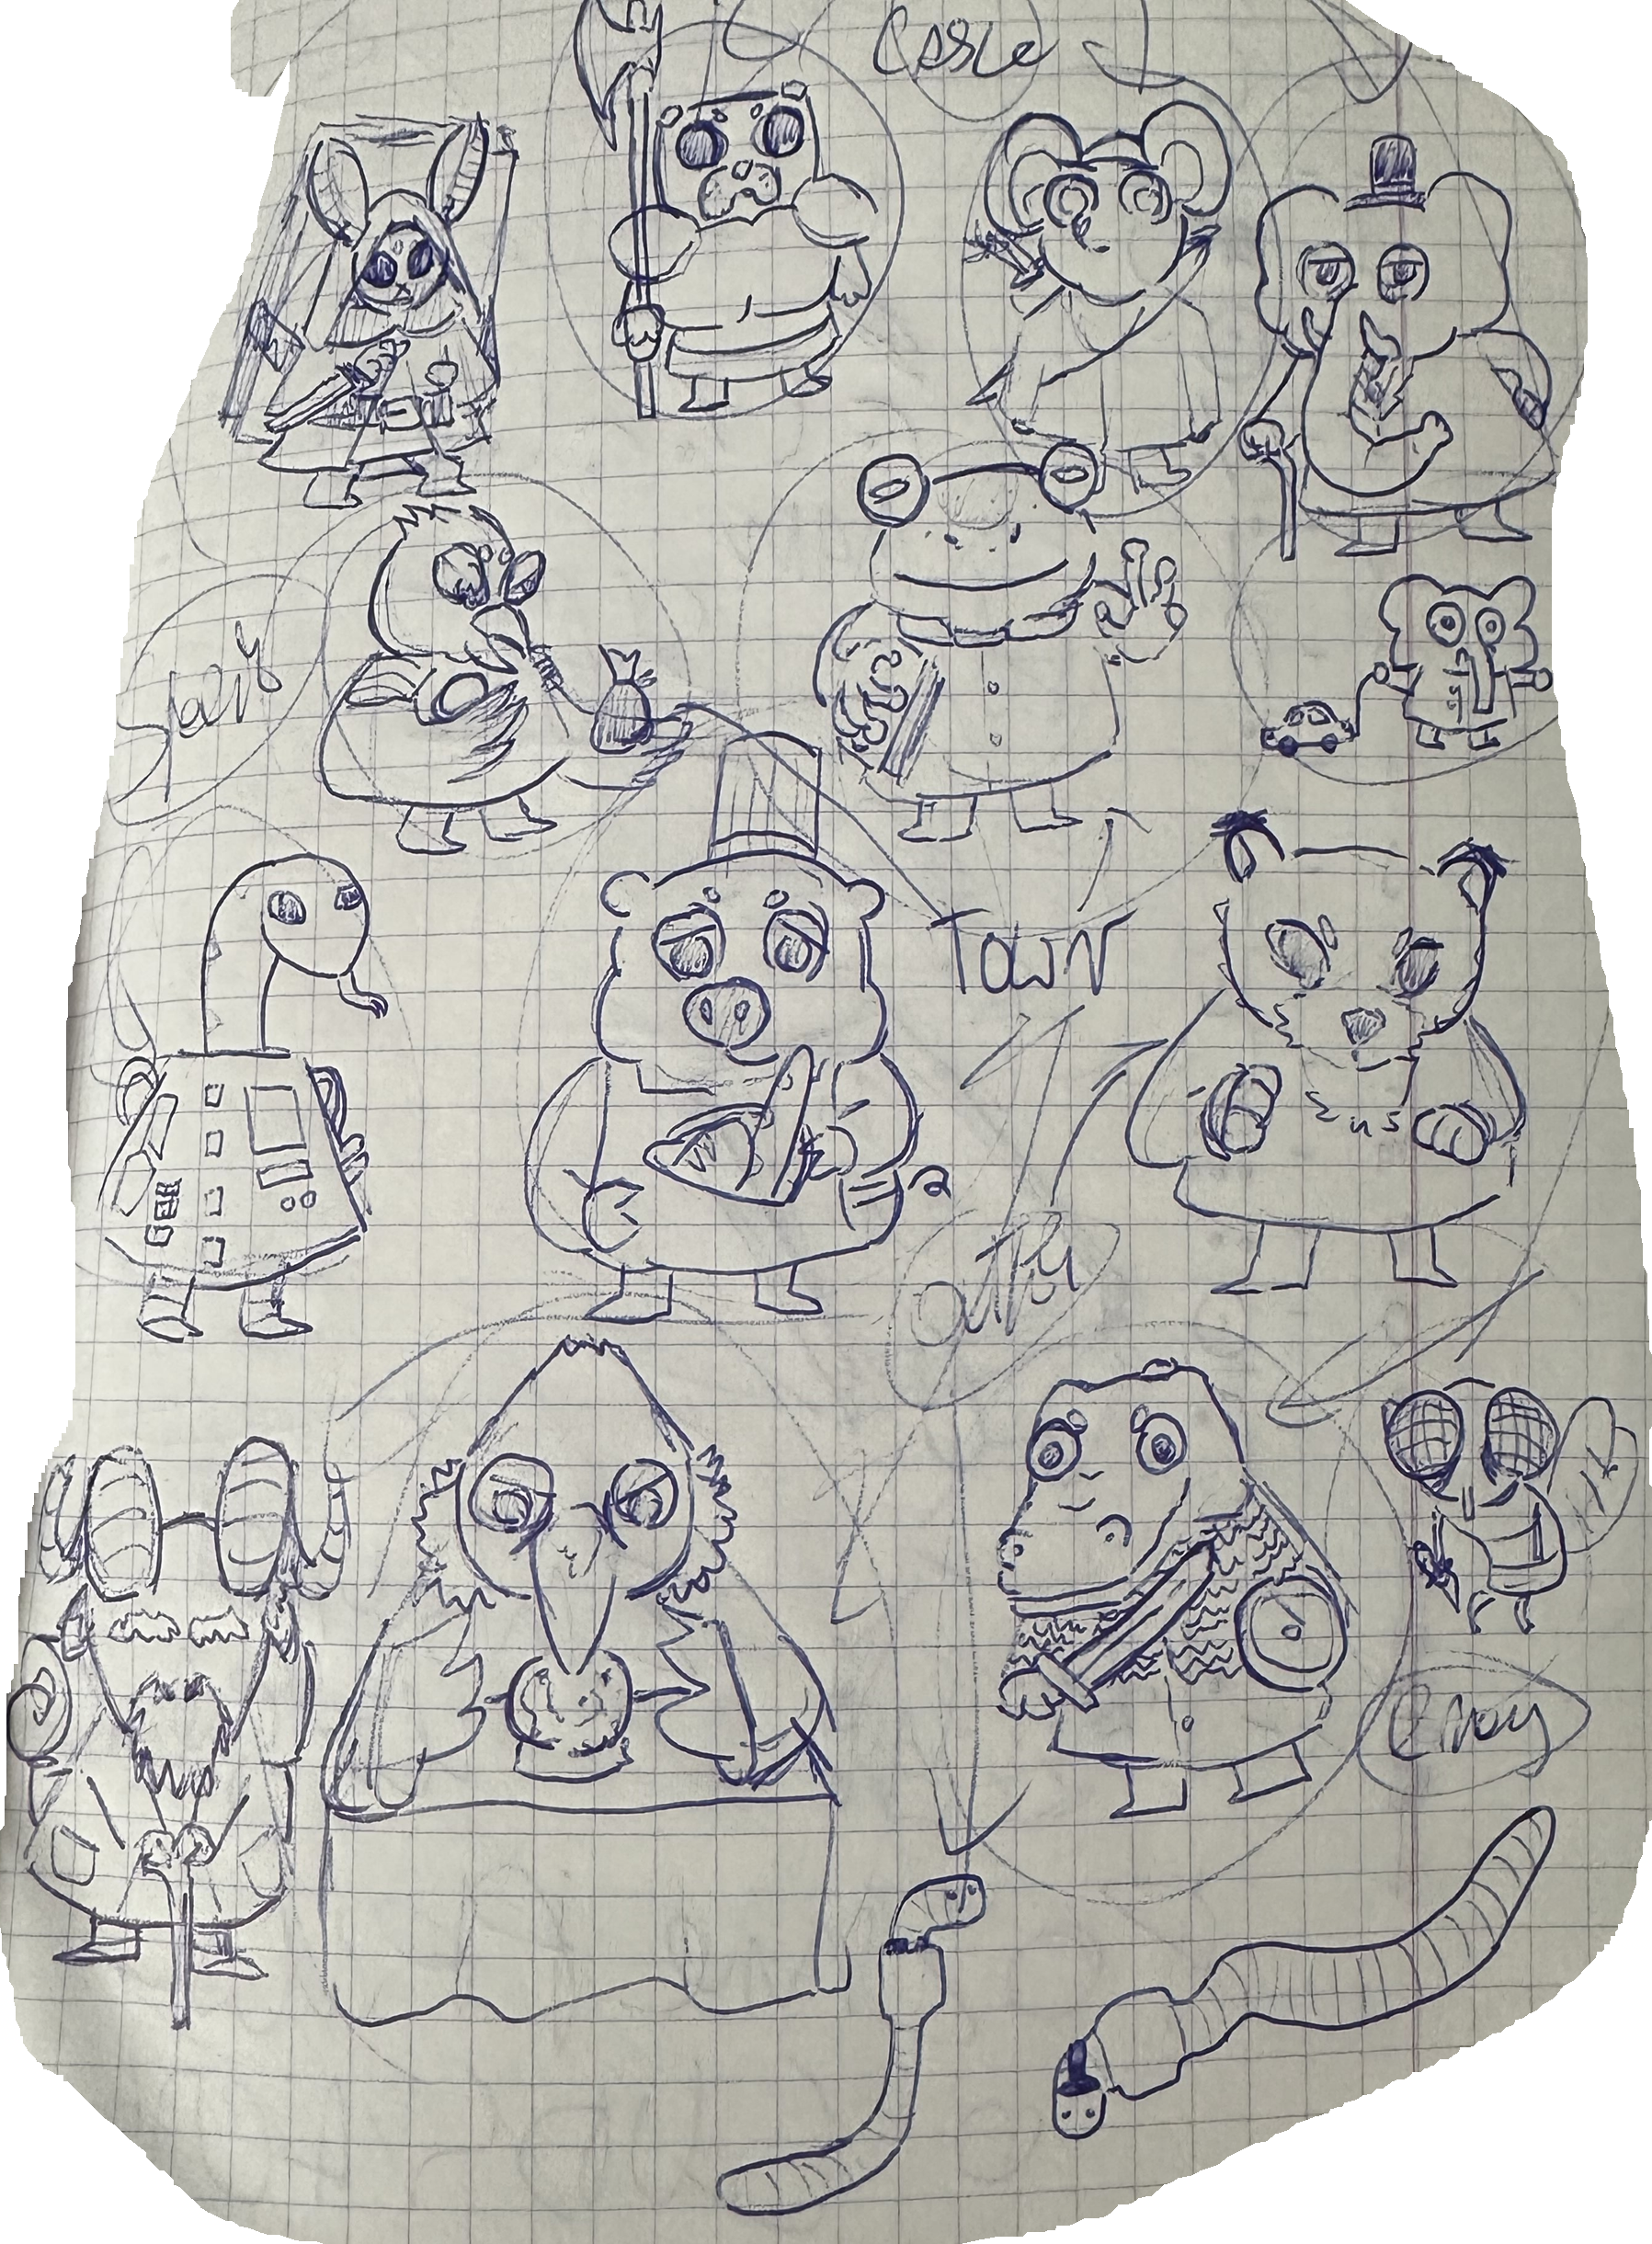
\includegraphics[width=0.75\textwidth]{images/npcs.png}
    \caption{Źródło własne: Szkic wstępny postaci niegrywalnych względem miejsca akcji.}
    \label{fig:npcs}
\end{figure}

\section{Decyzje Artystyczne}
%----------------------------------------------------------------------

\subsection{Styl Graficzny}

Gra utrzymana jest w ręcznie rysowanym stylu 2D, inspirowanym animacją zachodnioeuropejską i japońskim mangą. Kluczowe cechy stylu to:
\begin{itemize}
    \item Wyraźne, grube linie konturowe,
    \item Ograniczona, spójna paleta kolorów dla każdej lokacji,
    \item Ekspresyjne, stylizowane proporcje postaci,
    \item Dynamiczne sprite'y animowane klatka po klatce.
\end{itemize}

\subsection{Interfejs Użytkownika (UI)}

UI zaprojektowany jest tak, aby nie przesłaniać świata gry, a jednocześnie dostarczać graczowi wszystkich niezbędnych informacji. Składa się z:
\begin{itemize}
    \item \textbf{Paska HUD} – wyświetlającego zdrowie, siłę i licznik aktywnych wrogów,
    \item \textbf{Menu Ekwipunku} – systemu drag-and-drop do zarządzania przedmiotami i wyposażeniem,
    \item \textbf{Menu Questów} – panelu z listą aktywnych zadań głównych i pobocznych,
    \item \textbf{Ekranów Kontekstowych} – okien wygranej, przegranej, pauzy i nagrody.
\end{itemize}

\subsection{Muzyka i Dźwięk}

Oprawa audio planowana jest w stylu orkiestrowym z elementami ambientu. Każda lokacja będzie posiadać unikalny motyw muzyczny, a efekty dźwiękowe będą nagrane i przetworzone w FL Studio. Celem jest stworzenie atmosferycznej ścieżki dźwiękowej podkreślającej tajemniczość i melancholię tytułu \textit{Vanitas} – motywu przemijalności i marności.

\section{Diagram Przebiegu Rozgrywki}
%----------------------------------------------------------------------

Rozgrywka w \textit{Echoes of Vanitas} przebiega według następującego schematu:

\begin{enumerate}
    \item Gracz eksploruje świat gry, poruszając się postacią Nietoperza.
    \item W lokacjach natrafia na NPC dający questy – po wejściu w zasięg i wciśnięciu klawisza interakcji quest jest przyjmowany.
    \item Questy wymagają wykonania celów: zabicia określonej liczby wrogów (\textit{Kill}), zebrania przedmiotów (\textit{Collect}), dotarcia do lokacji (\textit{ReachArea}) lub rozmowy z NPC (\textit{Talk}).
    \item Po ukończeniu zadania gracz otrzymuje nagrody (złoto, doświadczenie, przedmioty).
    \item Zdobyte przedmioty mogą być wyposażone, ulepszane lub wyrzucone.
    \item Pokonanie wszystkich wrogów w lokacji powoduje wyświetlenie ekranu zwycięstwa.
\end{enumerate}
